\chapter{Research methodology}
\label{ch:methodology}

The aim of this research was to produce a technology-based solution to the problem of non-contact emotion detection within the context of games research. The solution is a method composed of a user-tailored model that is trained from a game-based calibration phase and is able to infer the emotional state of a player regarding stress and boredom via analysis of remotely acquired user signals. The constructs, models and methods involved in such aim have been individually studied in previous research, however the combination of all those elements in a single solution within the context of games research is novel. The utilization of those elements in combination was not yet demonstrated to work, so an iterative and incremental process must have been conducted to identify challenges, problems and solutions to achieve the desired goal.

\begin{figure}[h]
    \centering
    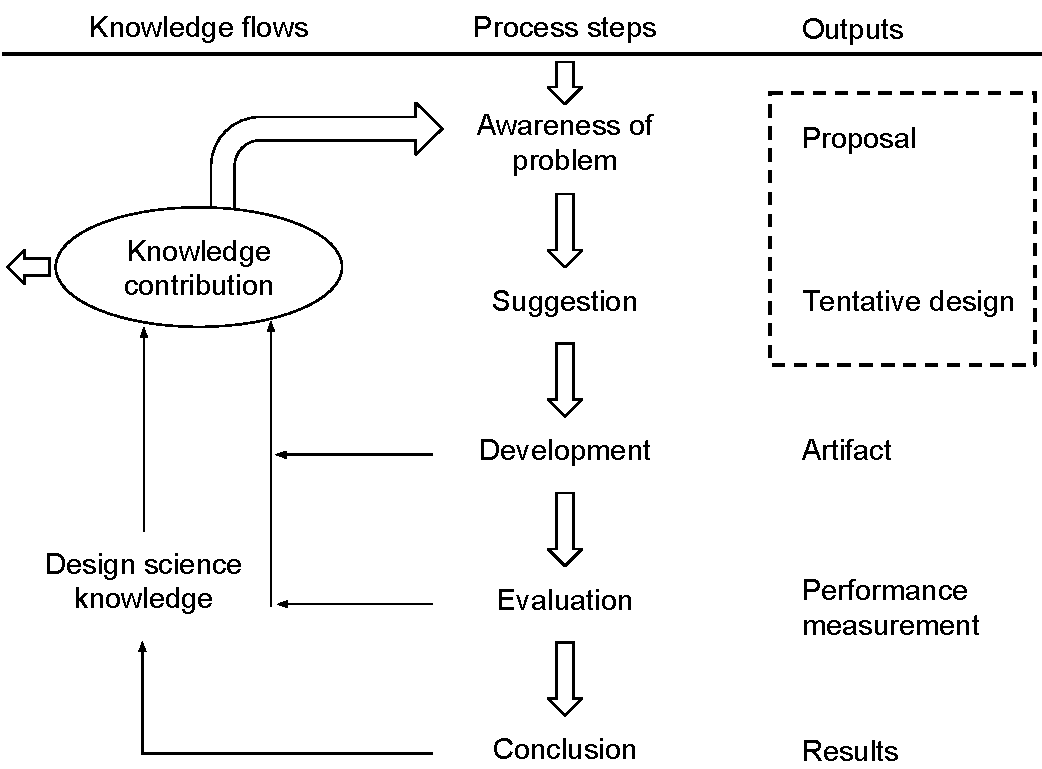
\includegraphics[width=0.9\textwidth]{Content/figures/vaishnavi-design-science-process-model}
    \caption{Design science research process model. Adapted from \textcite{vaishnavi2015design}.}
    \label{fig:vaishnavi-design-science-process-model}
\end{figure}

A research methodology that fits such iterative process is Design Science Research (DSR). Typically DSR is a problem solving process focused on developing new artifacts. \textcite{hevner2004design} defines design science in the context of Information Systems as a process that explores a relevant problem within an environment, iteratively measuring and refining the proposed solution according to the existing body of knowledge. The progress is made iteratively as the scope of the design of the artifact is expanded based on the discovery of available means, ends and constraints. Similarly \textcite{johannesson2014introduction} define design science as the scientific study and creation of artifacts as they are developed and used by people with the goal of solving practical problems of general interest. The outcome of DSR includes the contextual knowledge about the artifacts.

\textcite{vaishnavi2015design} structure the mentioned iterative process in five steps, illustrated in Figure \ref{fig:vaishnavi-design-science-process-model}: awareness, suggestion, development, evaluation and conclusion. They are the DSR process model, or DSR cycle. The awareness step is the recognition and articulation of a problem from an environment, which can be originated from studying the existing literature, for instance. The suggestion step presents a tentative design of how the problem might be addressed, which envisions a new functional artifact with a novel configuration of existing and/or new elements. The development and the evaluation steps comprehend the implementation of the tentative design and its analysis with well defined metrics and measurements. The evaluation either confirms or contradicts hypothesis about the behavior of the object, leading to new awareness (and other iteration of the process) or to a conclusion. Finally the conclusion step determines why and how the artifact worked or did not work within its environment. \textcite{vaishnavi2015design} categorize the knowledge that is gained during the research process and presented in the conclusion step as \textit{firm} and as \textit{loose ends}. In the former the conclusion shows facts that can be repeatably applied or behavior that can be repeatably invoked, while in the later the conclusion shows anomalous behavior that defies explanation and may serve as further research topics.

Types of artifacts resulting from DSR are constructs, models, methods and/or instantiations \parencite{oates2005researching,johannesson2014introduction}. Constructs are the terms, concepts, definitions and notations required to formulate and represent the problem. Models are a combination of constructs related to each other to represent possible solutions to a problem. Methods provide guidance on the models to be produced and the process to solve the problem. Finally instantiation is a working system that demonstrates that theories and artifacts, i.e constructs, models and methods, can be implemented in a computer-based system.

\begin{figure}[h]
    \centering
    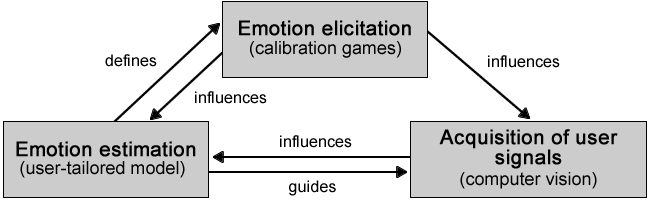
\includegraphics[width=0.8\textwidth]{Content/figures/method-components-dependency}
    \caption{Dependency among the main parts of this research: emotion elicitation, acquisition of user signals and emotion estimation.}
    \label{fig:method-components-dependency}
\end{figure}

The present research involved the use and orchestration of three main components, illustrated in Figure \ref{fig:method-components-dependency}. Those components are a game-based emotion elicitation part, composed of calibration games, the part involving remote acquisition of user signals via computer vision, and an emotion estimation part, composed of a machine learning model. The use of game-based material in a calibration phase in this research influences how users behave during the emotion elicitation process, e.g. body movement and facial expression. The movement of users directly impacts the techniques for remote extraction of user signals during both the calibration phase and the emotion estimation phase, since those techniques are highly influenced by motion. The accuracy of those techniques regarding the remotely acquired signals is affected as well, which might invalidate the feasibility of remotely reading determined physiological and non-physiological signals required by the emotion estimation model.

The interaction among the mentioned components, i.e. emotion elicitation, acquisition of user signals and emotion estimation, must be continuously investigated and adapted to overcome the previously described challenges. As a consequence, an iterative cycle of development and research is required, as illustrated by Figure \ref{fig:hevner-generate-test}. In each iteration, a possible solution for the current set of problems is generated, rigorously tested and evaluated, producing information to guide the next iterations in the cycle. The set of design alternatives in this research were related to the identification of physiological and non-physiological signals to be used in the emotion estimation process, how they can be elicited with games in a calibration phase, which computer vision techniques can be employed to remotely acquire the signals and which machine learning model is able to map the information into emotional states. The set of constraints involve problems associated with users behaving naturally, e.g. laughing and moving the body during the procedure, use of non-specialized hardware, e.g. ordinary camera, accuracy and efficiency of the solution, among others.

\begin{figure}[h]
    \centering
    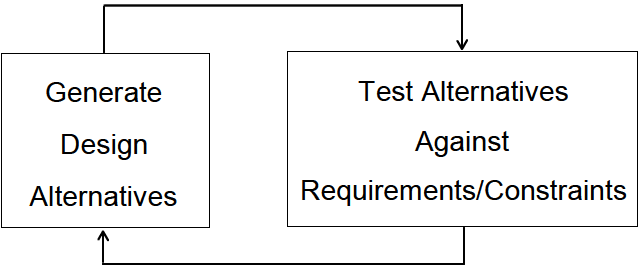
\includegraphics[width=0.8\textwidth]{Content/figures/hevner-generate-test}
    \caption{The Generate/Test cycle. Adapted from \textcite{hevner2004design}}
    \label{fig:hevner-generate-test}
\end{figure}

%The aim of this research is to produce a utility tool, i.e. software, which is an artifact based on a model built on existing theories, which will be combined in a new and innovative way. Since the result of the research is a model, which will be built from different measurements to predict or infer a state, the present work stands on the positivism paradigm. Essentially this work will formulate a theory about how the variation of physiological signals relate to stress/boredom levels in the context of games and how it can be remotely detected. The involvement of humans in the process might relate to the social side of interpretivism, however the foundation of the work is still based on the analysis of physiological signals. Such signals and their patterns might be different for each person, however they are still ordered and regular under the human being perspective. As a consequence, they can be objectively observed, measured and analysed with a quantitative approach and hypothesis testing.

Design-science research requires the application of rigorous methods in both the construction and evaluation of the designed artifacts \parencite{hevner2004design, johannesson2014introduction, oates2005researching}. One of such evaluation methods is experimental research, which is the strategy used to build and validate the knowledge in this thesis. Such approach is composed of a set of research designs that use controlled testing and manipulation of variables in order to understand causal processes \parencite{robson2016real}. The foundation of an experiment is to manipulate a variable (or a set of them) and measure any changes in other variables. It establishes the effect on a dependent variable, which is the focus of the research. The method constructed in this research links the variations of user signals to emotional states of stress and boredom in the context of games. Consequentially there is a causal effect in the process since identified variations (cause) will precede changes in stress/boredom levels (effect). It progresses to the construction of a hypothesis where the cause will consistently lead to the same effect so the link between variations of signals and emotional levels can be inferred or predicted.

The preferred experimental design for the present research was based on a within-subject approach \parencite{lane2015online}. In such approach, all participants perform at all levels of the treatment and there are no control groups.
%It is the opposite of a between-subjects approach, where subjects are divided in more than one group that receive different treatments. In that approach there are special groups, called control groups, that receive no treatment. The comparison between the control groups and the treatment groups ensures internal validity.
Such design could be criticized for having low internal validity, since it is not possible to unambiguously attribute cause and effect \parencite{kirk1982experimental}. A two-group approach could be suggested as having stronger internal validity, since it contains a control group and allows a less ambiguous conclusion. In the context of the present research, however, any multiple group design implies the comparison of physiological signals and emotional perceptions among different people. Given the social and cultural background of the participants, it is virtually impossible to compare two groups of people regarding stress/boredom. People have different preferences, culture and expectations, which cause maturation and history threats to internal validity \parencite{trochim2001research}.
%Additionally the process of comparing variations of physiological signals among different subjects is a complex task, even when subjects are similar, e.g. same age and sex. As a consequence, a subject in a control group might present a set of variations of signals and classify a game as boring, while a similar subject in another group might classify the same game as not boring at all, presenting a different set of variations of signals.
In that light, the within-subject approach relies on a one-group experimental design to increase internal validity, since subjects are compared with themselves, which removes inter-subject differences.

Design science research was the adequate approach for the research presented in this thesis. The iterative nature of the methodology allowed the investigation, validation and better understanding of the interactions among the components involved in the proposed research aim. The research presented in this thesis produced one main artifact, i.e. game-based, user-tailored method for estimation of emotions remotely. The artifact was produced from six iterations performed following the DSR cycle illustrated in Figure \ref{fig:vaishnavi-design-science-process-model}. Chapter \ref{ch:experiment1} documents five of those iterations, which were focused on proposing a solution for the dependency among the main parts of this research: emotion elicitation, acquisition of user signals and emotion estimation, as previously mentioned and illustrated in Figure \ref{fig:method-components-dependency}. Section \ref{sec:experiment1-study5}, in particular, details the iteration that produced the final tentative design that is the result of this thesis. The main artifact was composed of several different components, e.g. facial analysis and rPPG estimation of HR, that were orchestrated together to produce a game-based method for emotion estimation. Finally Chapter \ref{ch:experiment2} presents the final iteration in the DSR cycle. In that iteration a complete evaluation of the tentative design was performed. It produced several performance measurements that are presented and discussed in Section \ref{sec:experiment2-results} and Chapter \ref{ch:discussion}.

\section{Ethics and privacy in this research}
\label{sec:ethics-this-research}

The research presented in this thesis involved several elements that are sensitive to ethics and privacy, including how the research was conducted. This research involved two experiments and several studies conducted on the data gathered from those experiments. All experiments, as well the aforementioned analysis and data collection, were ethically conducted and handled according to the \textit{Principals for Research Ethics in the Humanities and Social Science}\footnote{\textit{Forskningsetiska Principer inom Humanistisk-Samhällsvetenskaplig Forskning}}. Particularly all materials and procedures were designed after recommendations of the CODEX\footnote{http://www.codex.vr.se}, the Swedish Research Council, which provides guidelines, ethics codes and laws that regulate and place ethical demands on the research process.

Following such guidelines, participants of the aforementioned experiments had given a written consent stating that they understood what was happening and that they voluntarily wanted to participate in the study being conducted. Participants were informed that they may choose not to participate and they may withdraw their consent to participate at any time. In such case, they would not be asked for any explanations if they decide not to participate or to withdraw from any activity. Additionally subjects were informed regarding the description of the research, including the overall research plan and the aim of the research being conducted. A main component of this research is the idea of calibration games, which are games whose difficulty level continually progresses over time to induce stress. It is important to state and clarify that such induced emotional state of stress comes from the addition or speed up of game elements that the subject needs to handle, e.g. more cards to sort or faster falling pieces. Both the content and theme of all games used in this research are casual, family friendly and are completely based on cartoon graphics. No severe emotional or traumatizing stress was induced, only the expected level of stress resulted from the ordinary interaction with a game whose elements change, i.e. intensity in the activity on screen. In no circumstance offensive, violent, culturally or morally disturbing content was used in the games, e.g. guns and gore, to induce any emotional state. The games used in this research are not different than any existing commercial game whose difficulty level also increases to induce stress in order to produce a feeling of reward when the player completes a challenge. As described in Chapters \ref{ch:experiment1} and \ref{ch:experiment2} (on pages \pageref{ch:experiment1} and \pageref{ch:experiment2}, respectively), before starting any experiment, subjects were instructed to not give up in the middle of the games. Such instruction was contextualized with the games to be played and it never superseded or prevented the subjects from interrupting the activity at hand and leaving the study, as they were informed they could do, even during the time they were playing the games. As previously mentioned, subjects were informed in more than one occasion that they could stop any activity and quit the study at any time. In light of that, it was deemed that no further actions regarding ethical considerations were needed since the experiments only included normal interaction with standard technology.

Data privacy issues were also made clear to all participants, e.g. session being video-recorded, and all efforts were put in place to assure the participants privacy. For instance, participants were informed beforehand about which information was being collected from them, e.g. HR, video, in-game actions and answers to questionnaires. They were informed that the collected data would only be used for non-commercial research purposes, that all collected data would be stored off-line in a hard-drive that was only accessible by the principal investigator. Data protection included restrict access to such hard-drive, which was handled and keep physically under the principal investigator's possession at the dependencies of the University of Sk\"ovde. It helped ensure that unauthorized persons would not have access to the data. All participants were also informed beforehand that all data was anonymously collected and their identity would not be revealed, including in any publication resulting from this work. It is not possible to trace any published results or the information in the present thesis back to the subjects. Subjects were assured that their data would never be publicly disclosed, i.e. videos, HR information, pictures and answers to questionnaires, without their written consent. Some of the publications of this research presented pictures of participants, which were contacted in advance and asked for an authorization regarding the use of such pictures.

Finally in order to ensure subjects fully understood the research being conducted and how their data would be used, in both experiments each subject attended a debriefing session. In such session, the researcher explained to subjects how the games just played by them were designed, including the linear progression of boredom and stress. Additionally subjects were informed regarding how the data would be analyzed, e.g. find a relation between HR and stressful moments, or that remote estimations of their HR would be performed on the video recordings and tested against the data collected by the watch participants used. Participants had the opportunity to ask questions about the experiment, the study, the data collection or any matter related to the research they deemed important. It is also important to highlight that a wearable sport device, i.e. watch (TomTom Cardio Runner), has been used in this research. Such device was selected in favor of a medical grade equipment to reduce privacy and ethical concerns regarding data gathering of personal biological information.

%\section{Research objectives}

%The objective of this research is to produce a method that is able to interpret remotely acquired signals from a person playing a game and detect his/her current emotional state regarding stress and boredom according to data previously obtained in a calibration phase. The model will be implemented in a software that uses a video feed to detect the person's emotional state.

%The current approaches used to obtain information from the players during games research inevitably affect the player's experience. They require the user to stop the game activity in order to share his/her current state, such as by answering a questionnaire. The frequency that such questionnaires are issued is also a concern. If performed too often, more information might be collected, but the data might contain noise caused by the frequent interruptions, e.g. player is more stressed/bored by the questionnaire interruptions than by the game itself. If performed too sparse, not enough information will be gathered from the player. A physical sensor attached to a player, on the contrary, allows a continuous monitoring process, however it is intrusive and might interfere with the player capacity to interact with the game. It might prevent the use or movement of specific parts of the body, for instance. Physical sensors also increase the chances of the player to behave differently as a side-effect of the monitoring process itself.

%A purely remote-based solution, as the one proposed by this research, enhances the tooling available to the games research community regarding investigation methods of stress and boredom. A games researcher will be able to increase the internal validity of his/her workflow by ensuring the player keeps the focus on the game without interruptions and by minimizing the side effects (and inconveniences) of physical monitoring. This research could also be deployed as a solution for game developer studios to automatically analyze hours of recorded gameplay and highlight the moments when boredom/stress levels changed significantly. As a complement the solution will be based on a single, ordinary camera and a software implementation, which eliminates the use of complex setups of physical sensors. It eases the investigation process and reduces costs.
